\documentclass{cshwk}

\title{HW \#3, Chapter 3}

\begin{document}
\maketitle

\section*{Chapter 3, P37.}

Compare GBN, SR, and TCP (no delayed ACK). Assume that the timeout values for all three protocols are sufficiently long such that 5 consecutive data segments and their corresponding ACKs can be received (if not lost in the channel) by the receiving host (Host B) and the sending host (Host A) respectively. Suppose Host A sends 5 data segments to Host B, and the 2nd segment (sent from A) is lost. In the end, all 5 data segments have been correctly received by Host B.

\begin{enumerate}
    \item[a.] How many segments has Host A sent in total and how many ACKs has Host B sent in total? What are their sequence numbers? Answer this question for all three protocols.
    \item[b.] If the timeout values for all three protocols are much longer than 5 RTT, then which protocol successfully delivers all five data segments in the shortest time interval?
\end{enumerate}

\subsection*{Solutions}
\begin{figure}[htbp]
    \centering
    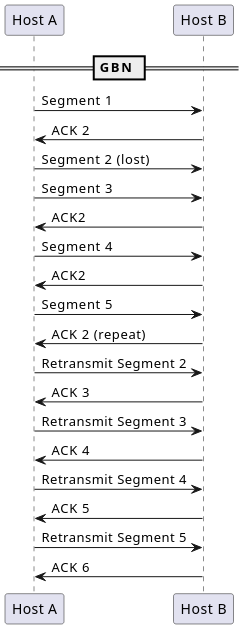
\includegraphics[width=0.2\textwidth]{hw3-4-1.png}
    \caption{GBN Protocol}
    \label{fig:gbn}
\end{figure}

\paragraph{a.} In GBN protocol, The packets are send as shown in the Fig.~\ref{fig:gbn}.

As shown in the figure, \textbf{Host A sends 8 data segments to Host B.} They are the first 1-5 segments and the retransmission of the 2-5 segments. \textbf{Host B sends 8 ACK packets to Host A. }

\begin{figure}[htbp]
    \centering
    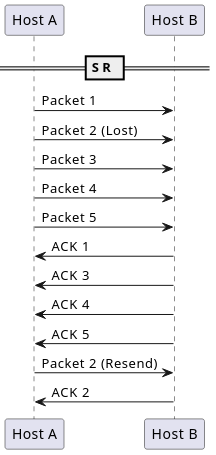
\includegraphics[width=0.2\textwidth]{hw3-4-2.png}
    \caption{SR Protocol}
    \label{fig:sr}
\end{figure}
In SR protocol, The packets are send as shown in the Fig.~\ref{fig:sr}. 

As shown in the figure, \textbf{Host A sends 6 data segments to Host B.} They are the first 1-5 segments and the retransmission of the 2 segment. \textbf{Host B sends 5 ACK packets to Host A. }

\begin{figure}[htbp]
    \centering
    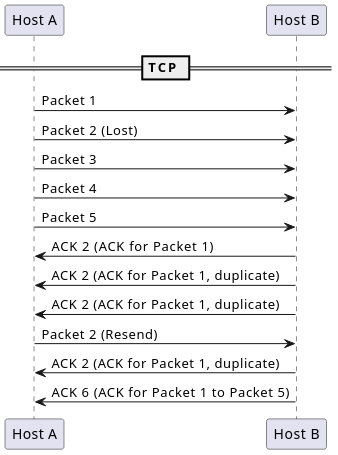
\includegraphics[width=0.3\textwidth]{hw3-4-3.png}
    \caption{TCP Protocol}
    \label{fig:tcp}
\end{figure}

In TCP protocol, The packets are send as shown in the Fig.~\ref{fig:tcp}.
As shown in the figure, \textbf{Host A sends 6 data segments to Host B.} They are the first 1-5 segments and the retransmission of the 2 segment. \textbf{Host B sends 5 ACK packets to Host A. } Notice that, TCP always sends an ACK for the expected sequence number.

\paragraph{b.} \textbf{TCP uses the shortest time} because it employs Fast Retransmit to recover lost segments without waiting for a timeout.

\end{document}